
\subsection{Изъятие предметов из сети хранилищ}

\textbf{Участники:}
Менеджер, Администратор, Заказчик.

\textbf{Описание:}
Заказчик договаривается с Менеджер об
изъятии предметов из конечного хранилища. Далее Менеджер 
создает в Системе заявку на изъятие предметов из 
хранилища А. Администратор хранилища либо подтверждает 
заявку на поставку предметов, либо отклоняет ее. В 
любом процесс прекращается уведомлением Менеджера и 
поставщика.

\begin{figure}[h]
  \centering
  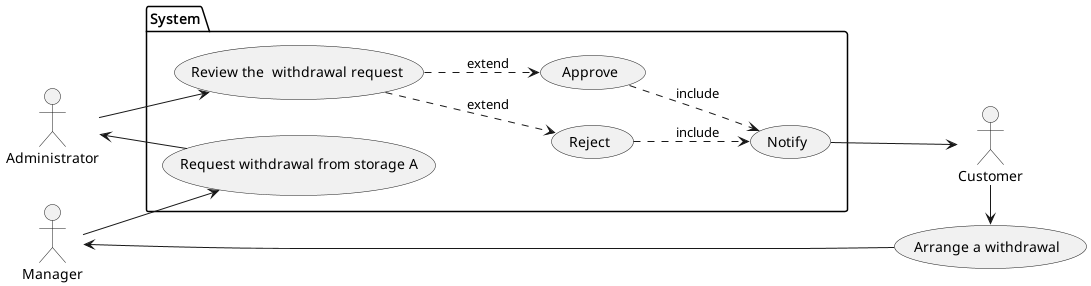
\includegraphics[width=12cm]{../../out/spec/figure/usecase/withdrawal_confirm/Storage Net, Use Case, Withdrawal.png}
  \caption{Use Case: Withdrawal}
\end{figure}
